\section{Marco teórico}
\subsection{Aprendizaje automático}
%- explicación resumida tipos de aprendizaje (supervisado, no supervisado, semisupervisado)
 Dentro de las diferentes ramas de la inteligencia artificial, los algoritmos utilizados se pueden clasificar en tres grandes ramas según la forma en que son entrenados: algoritmos de aprendizaje supervisado, algoritmos de aprendizaje semi-supervisado y algoritmos de aprendizaje no supervisado. Los primeros son los que se utilizan cuando para el conjunto de entrenamiento \(X\) se tiene un conjunto de etiquetas \(y\) con las que se relacionan unívocamente, y de esta manera, los algoritmos encuadrados dentro de esta rama se encargan de estimar una función que mapee los datos del conjunto \(X\) al conjunto \(y\), con el fin de  luego poder realizar inferencias a partir de sólo nuevos casos de entrada. Los algoritmos de aprendizaje no supervisado se utilizan en situaciones en las que se tiene un conjunto de datos de entrada \(X\) pero no se tiene un conjunto de etiquetas asignadas a estos datos, estos algoritmos se emplean para realizar sobre los datos tareas tales como agrupamientos, detección de anomalías, reducción de dimensionalidad, entre otras. Por último, la rama del aprendizaje semi-supervisado entra en juego para aquellos casos en los que se tiene un pequeño conjunto de datos etiquetado, y un gran conjunto de datos no etiquetados.
 
%- explicación profunda aprendizaje supervisado, ejemplos otros tipos de problemas
 En este trabajo se contará tanto con un conjunto de entrenamiento que serán bases de datos de imágenes como con sus pertenecientes etiquetas, por lo que se intentará mapear mediante algún algoritmo (en este caso técnicas de aprendizaje profundo) cada imagen con sus etiquetas: aprendizaje supervisado.
 
 Dentro de esta rama existen otros algoritmos que pueden servir para este problema o para otros problemas de dominio diferente como son los árboles de decisión, regresiones lineales o logísticas, ensembles, etc.
 
\subsection{Representación de una neurona}
%- explicación neurona
 En este trabajo, como bien se explicó anteriormente, se abordará la solución mediante técnicas de aprendizaje profundo, por lo que a continuación se dara lugar a las explicaciones pertinentes relacionadas a este tipo de técnica.
 Para empezar es necesario comentar que el término "profundo" recae en la profundidad de las redes neuronales que se utilizan en esta técnica. Estas redes pueden estar compuestas hasta por millones de neuronas interconectadas entre si; neuronas que se representan como se observa en la imagen \ref{fig:representacion_neurona} en donde se muestra un ejemplo de una neurona con \(n\) entradas, conformada por: 
 \begin{itemize}
 	\item Entradas: conjunto de datos de entrada \(x_1\)..\(x_n\)
 	\item Pesos: conjunto de pesos \(w_1\)..\(w_n\) correspondientes a cada entrada
 	\item Función de agregación: función que agrega la multiplicación pesada entre cada entrada \(x\) y su correspondiente peso \(w\).
	\item Función de activación: función no lineal responsable de mapear el resultado de la función de agregación en salidas (según que tipo de función los resultados son valores entre [0, 1]o [-1, 1]).
	\item Salida: resultado de la función de activación.
 \end{itemize}
 
 
\begin{figure}
\centering
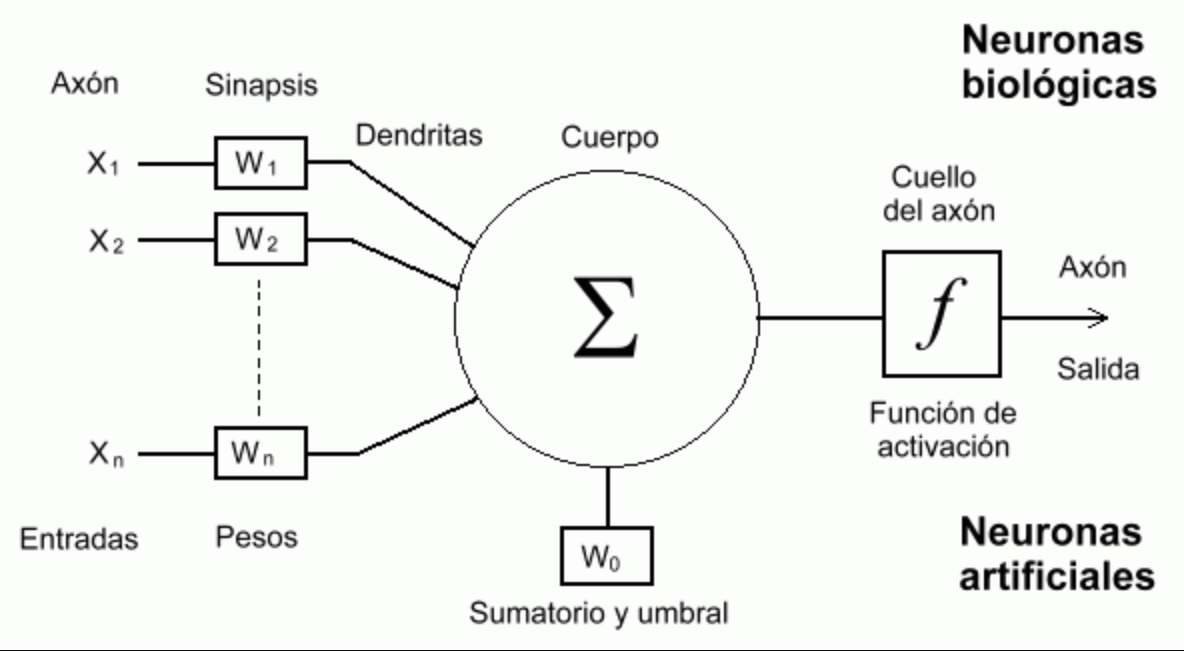
\includegraphics[width=0.7\linewidth]{images/representacion_neurona}
\caption[Representación de una neurona]{Representación de una neurona}
\label{fig:representacion_neurona}
\end{figure}

De esta manera, se puede obtener la salida de la neurona \(Y\), a partir de aplicar la función de activación \(\sigma\) a la suma entre el sesgo \(b\) y la multiplicación matricial del conjunto de entrenamiento \(X\) y los pesos \(W\).

\begin{equation}
Y=\sigma\left(W^{T} X+b\right)
\end{equation}


\subsection{Red Neuronal}\label{red_neuronal}

%- explicación redes neuronales profundas
 Una red neuronal, como su nombre lo enuncia, es una consecución de capas de \(N\) neuronas en cada una, conectadas entre sí como se puede ver en el ejemplo de la figura \ref{fig:redneuronal}. Es necesario que se cuente con capas de entrada, capas ocultas y capas de salida; para la figura \ref{fig:redneuronal} se tiene una capa de entrada, dos capas ocultas y una capa de salida. 
 El fin de las redes neuronales es aprender representaciones del contenido de la información en relación a las salidas esperadas para luego poder hacer inferencias en nuevo contenido, a modo de ejemplo, si se tienen imágenes de perros y gatos, y el fin es detectar si se trata de un perro o un gato la red posiblemente no aprenda las mismas representaciones que si el fin de la misma es detectar presencia o ausencia de animales.
 
 
 \begin{figure}
 	\centering
 	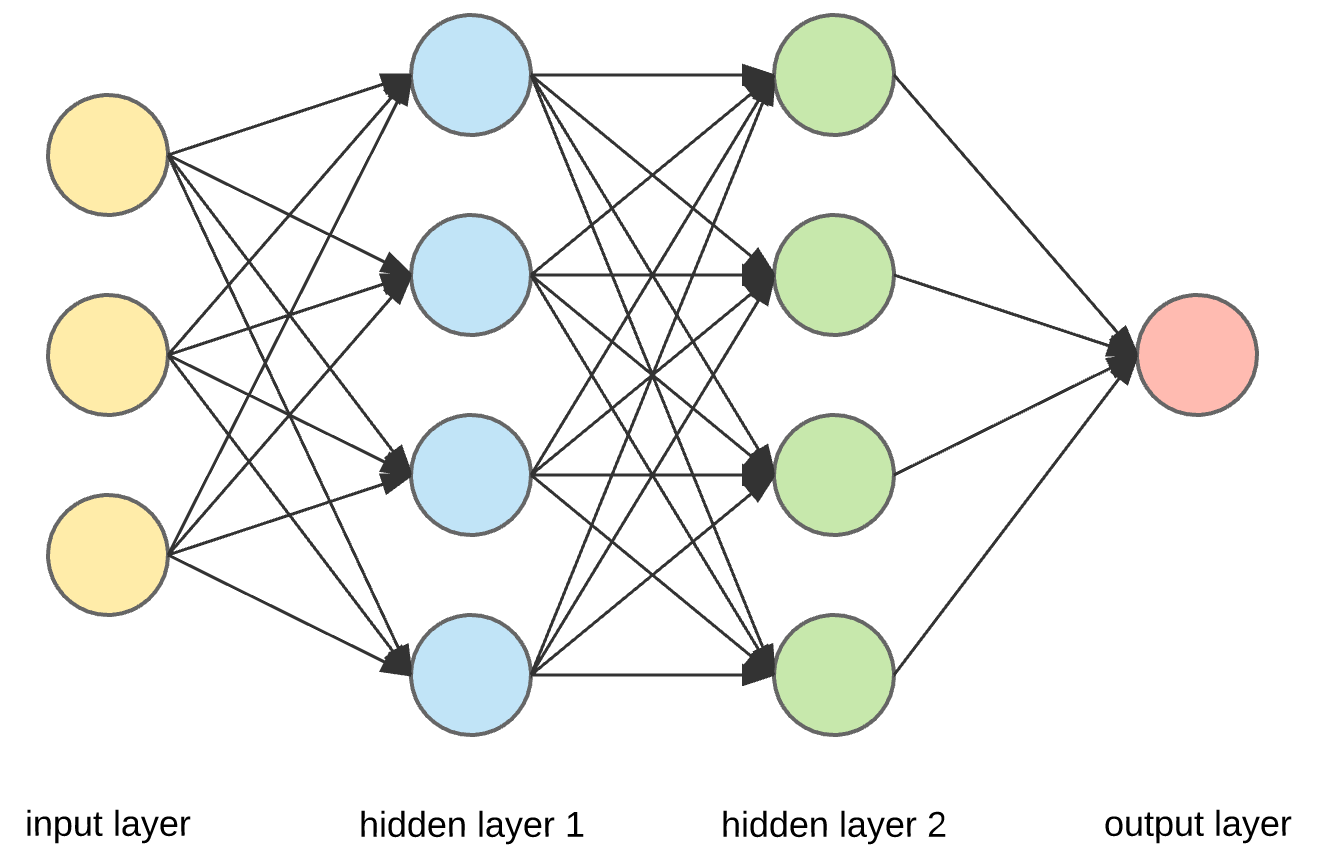
\includegraphics[width=0.7\linewidth]{images/red_neuronal}
 	\caption[Ejemplo red neuronal]{Perceptrón Multi Capa}
 	\label{fig:redneuronal}
 \end{figure}

 Para explicar el funcionamiento de las redes neuronales es necesario también introducir algunos conceptos como son la propagación hacia adelante y hacia atrás, función de pérdida y optimización. Durante la fase de entrenamiento, los pasos que se siguen son:
 \begin{enumerate}
 	\item Inicialización de pesos y sesgo
 	\item Propagación hacia adelante
 	\item Evaluación de función de pérdida
 	\item Propagación hacia atrás
 \end{enumerate}
 Antes de comenzar a usar la red, es necesario inicializar los pesos que conectan las capas, suele hacerse se hace de manera aleatoria a partir de una distribución normal, aunque existen otros métodos como hacerlo a partir de una distribución uniforme, la inicialización de Xavier, entre otras.
 
 La propagación hacia adelante es la actividad en que se le brindan los datos a la capa de entrada de la red para que se evalúen todas las capas en esa dirección aplicando \ref{formula:forward_prop} en cada capa tomando como entrada la capa inmediata anterior. De esta manera, se obtiene como salida de la red sus predicciones. 
 
 Luego, a partir de las salidas de la red es posible medir la función de pérdida que brinda la información de cuán cerca estuvo la red de predecir las salidas correctas y con la que se puede computar la propagación hacia atrás del error, es decir, optimizar la función de pérdida actualizando los pesos desde atrás hacia adelante teniendo en cuenta el error. La manera de hacerlo es mediante la derivada parcial de la función de costo con respecto tanto a los pesos \(\alpha\) como a los sesgos \(b\) en cada capa para conseguir un nuevo valor para \(W\) y \(b\).
  
 
 \begin{equation}\label{formula:forward_prop}
 z=W^{T} X+b
 \end{equation}
 
 \begin{equation}
 \omega:=\omega-\alpha \frac{\partial J(\omega, b)}{d \omega}
 \end{equation}
 
 \begin{equation}
 b:=b-\alpha \frac{d J(\omega, b)}{d b}
 \end{equation}
 
 
 
 Un problema común al entrenar una red es el sobreentrenamiento, que se da cuando la red sobreajusta sus pesos para el conjunto de entrenamiento y pierde capacidad de generalizar. Una forma facil de verificarlo es mediante un subconjunto de validación, que son imágenes que no se utilizan para entrenar la red sino que para medir realmente cómo está funcionando la misma. Para contrarrestar estas situaciones existen capas regularizadoras, es decir, que evitan la concetración de gran porcentaje del conocimiento en un conjunto de unidades de las capas y sean capaces de compartir lo más que se pueda la representación del contenido aprendido. Aunque existen otras, las más utilizadas son \(dropout\) y \(batch normalization\). La capa \(dropout\) se encarga de apagar conexiones aleatoriamente entre capas durante el entrenamiento, esto hace que no se entrene siempre con las mismas unidades dentro de cada capa, y que diferentes unidades se activen para una misma situación. La capa de \(batch normalization\) aplica una función de regularización que sale de la media y la varianza de cada bache durante el entrenamiento, agregando ruido en las activaciones y evitando que las activaciones no sean demasiado altas ni demasiado bajas reduciendo el desplazamiento covariable interno (\(internal covariance shift\), en inglés), y la manera de hacerlo es mediante la aplicación de las ecuaciones \ref{formula:bn_minibatch_mean}, \ref{formula:bn_minibatch_variance}, \ref{formula:bn_normalization}, \ref{formula:bn_scale_and_shift}, como se explica en el Algoritmo 1 de \cite{BatchNorm}
 
 \begin{equation}\label{formula:bn_minibatch_mean}
 \mu_{\mathcal{B}} \leftarrow \frac{1}{m} \sum_{i=1}^{m} x_{i}
\quad { // media del mini-batch}
 \end{equation}
 
 \begin{equation}\label{formula:bn_minibatch_variance}
 \sigma_{\mathcal{B}}^{2} \leftarrow \frac{1}{m} \sum_{i=1}^{m}\left(x_{i}-\mu_{\mathcal{B}}\right)^{2}
\quad { // varianza del mini-batch}
 \end{equation}
 
 \begin{equation}\label{formula:bn_normalization}
 \widehat{x}_{i} \leftarrow \frac{x_{i}-\mu_{\mathcal{B}}}{\sqrt{\sigma_{\mathcal{B}}^{2}+\epsilon}}
\quad { // normalización}
 \end{equation}
 
 \begin{equation}\label{formula:bn_scale_and_shift}
 y_{i} \leftarrow \gamma \widehat{x}_{i}+\beta \equiv \mathrm{B} \mathrm{N}_{\gamma, \beta}\left(x_{i}\right) {// escalación y desplazamiento}
 \end{equation}
  
 

%- explicacion funcionamiento:
%	- forward prop 
%	- back prop
%	- regularizers:
%		- dropout
%		- batch norm
	- optimizers
	- metrics
	- loss functions
	- activation functions
	
\subsection{Red Neuronal Convolucional}
%- explicación razón de convoluciones
Las redes neuronales convolucionales son una variante de las redes neuronales en las que la extracción de características se realiza mediante capas convolucionales. Fueron introducidas en \cite{lecun1995convolutional} por LeCun, Bengio y Yann, tres investigadores referentes en el mundo del aprendizaje automático y las redes neuronales, y han transformado la forma de resolver problemas de clasificación de imágenes desde entonces.

Como es posible observar en la figura \ref{fig:convolution}, una convolución es una operación matemática. Se puede entender como el resultado de aplicar un filtro (una matriz con forma \(N x N\)) en todas las regiones de la imagen con el fin de obtener una nueva. En el ejemplo se aprecia que el resultado de la aplicación del filtro en la esquina superior izquierda de la imagen se obtiene a partir de multiplicar cada valor del pixel en la imagen de entrada con su par en la misma posición en el filtro, finalmente en el ejemplo se tiene que el valor del nuevo pixel en la imagen de salida es \((-1 * 3) + (0 * 0) + (1 * 1) + (-2 * 2) + (0 * -6) + (2 * 2) + (-1 * 2) + (0 * 4) + (1 * 1) = -3 \). La operación detallada previamente se aplica a toda la imagen para obtener la imagen resultado, teniendo en cuenta tanto los valores del \(stride\) como del \(padding\) definidos para la capa. El parámetro \(stride\) define cada cuántos píxeles de la imagen de entrada se aplicará el filtro, mientras que mediante el parámetro \(padding\) se decide cómo se tratarán los bordes, esto es debido a que existen ocasiones en las que se desea obtener una imagen en la que se le apliquen convoluciones también a los bordes de la misma y las formas más comunes de hacerlo son agregando a los bordes \(N\)) pixeles más (dependiendo del \(stride\)), ya sea con ceros o el mismo valor de sus píxeles más cercanos. 

Gracias a la aplicación de estas capas las redes convolucionales son capaces de aprender representaciones del contenido invariantes, ya que cada filtro se aplica a todas las subregiones de la imagen haciendo que su aprendizaje se base en las imágenes completas. A continuación se detallará una red convolucional en funcionamiento, con el fin de mostrar cómo estas capas se interconectan entre sí, reducen las representaciones computadas y finalmente se conectan con el fin de realizar inferencia con lo aprendido. Como se mostrará a continuación existen muchas configuraciones de redes neuronales convolucionales, aunque para simplificar la explicación se utilizará la red detallada en la figura [TODO> AGREGAR FIG CON RED SIMPLE (conv, maxpooling, conv, maxpooling, fc, dropout, softmax)]. Para comenzar, una capa de entrada es necesaria, en este caso (al igual que en el presente trabajo) serán imágenes en formato RGB normalizadas, es decir, una matriz de \(ALTO x ANCHO x CANALES(3)\) por cada imagen; luego esta entrada será convolucionada aplicando la operación matemática previamente explicada y sus salidas serán agrupadas por una capa llamada \(pooling\), en esta capa se buscará reducir tanto las representaciones aprendidas como la cantidad de cálculos a realizar: se agruparán mediante la aplicación de un filtro \(f\) y un método \(M\) los resultados de la convolución, siendo \(f\) una matriz (usualmente de \(2 x 2\)) y \(M\) utilizar la media o el máximo de los valores de la convolución en cada sector en que se aplique el filtro, al igual que en la convolución se aplica en toda la imagen, aunque tiene dos diferencias fundamentales: no tiene parámetros que aprender o ajustar y busca reducir las representaciones a matrices de menor orden. Continuando con la red, aplica nuevamente una convolución seguida de una capa de pooling que se conecta a una capa totalmente conectada (la misma que se utiliza en el perceptrón multicapa). Antes de llegar a la capa de predicciones, la capa totalmente conectada se conecta a una de dropout que se encarga de apagar conexiones entre neuronas de dos capas contiguas aleatoriamente durante el entrenamiento con el fin de ayudar a que el conocimiento no quede sólo en algunas de éstas. Finalmente, la capa de dropout se conecta con una capa de salida que se encargará de devolver las probabilidades con las que se predice cada clase (básicamente, una capa totalmente conectada con función de activación como las mencionadas en \ref{red_neuronal}).

\begin{figure}
	\centering
	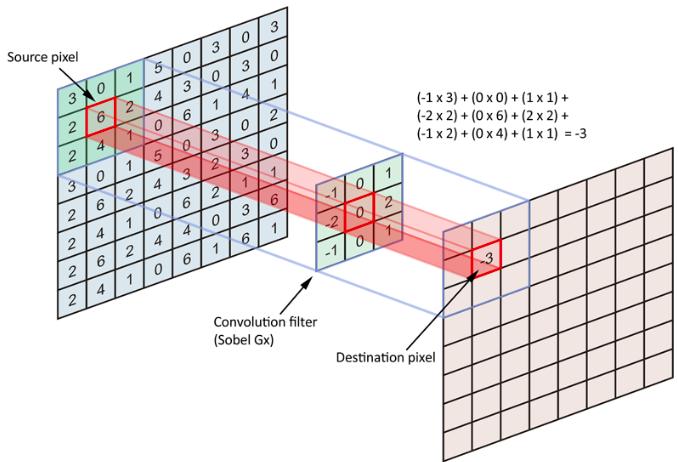
\includegraphics[width=0.7\linewidth]{images/convolution}
	\caption[Convolución]{Convolución}
	\label{fig:convolution}
\end{figure}

%- partes:
%	- Convolución
%	- stride
%	- pooling layers
- ejemplo simple

\subsection{Redes preentrenadas y Aprendizaje por transferencia} 

% Redes preentrenadas
Como entrenar redes neuronales profundas resulta muy costoso computacionalmente tanto por la profundidad como por la cantidad de datos con las que se las necesita entrenar, con el pasar del tiempo quienes tienen accesso a capacidad de cómputo comenzaron a liberar redes entrenadas con diferentes bases de datos. Posiblemente, las redes liberadas más conocidas sean las que se entrenaron utilizando ImageNet \cite{ImageNet}, una base de datos de 3.2 millones imágenes centradas en objetos, aunque también existen otras bases de datos de imágenes abiertas como son COCO Dataset \cite{BMVC2015_52}, Places Dataset \cite{learning_deep_features}, etc.

%- Transfer Learning
En la actualidad existen redes preentrenadas con diferentes arquitecturas y datasets como son VGGNet (figura \ref{fig:vgg16}), InceptionNet (figura \ref{fig:googlenet}), DenseNet, ResNet, Bert, GPT2 (figura \ref{fig:gpt2}). Dependiendo el tipo de problema y la base de datos con la que fue entrenada cada red, es posible tomar provecho de las mismas, ya sea aplicando reentrenamiento en ellas o no.
\begin{figure}
	\centering
	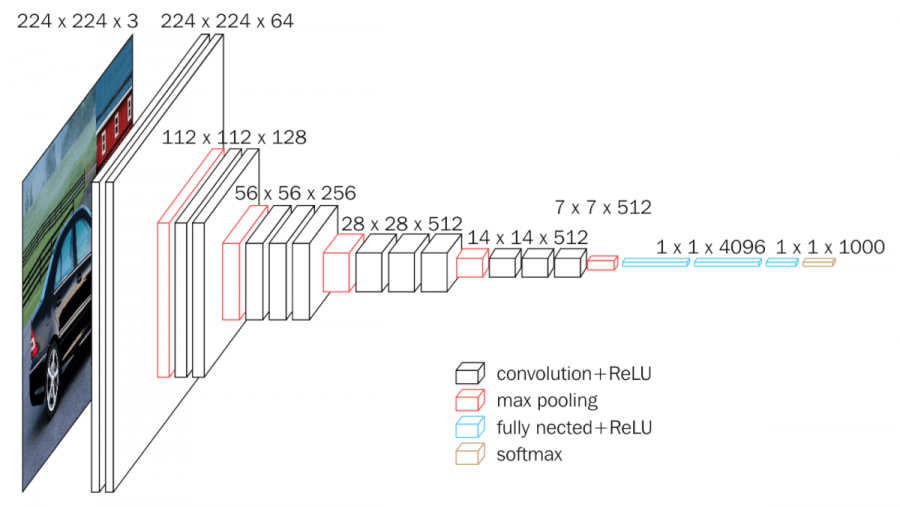
\includegraphics[width=1\linewidth]{images/vgg16}
	\caption[Arquitectura VGG16]{Arquitectura VGG16}
	\label{fig:vgg16}
\end{figure}

\begin{figure}
	\centering
	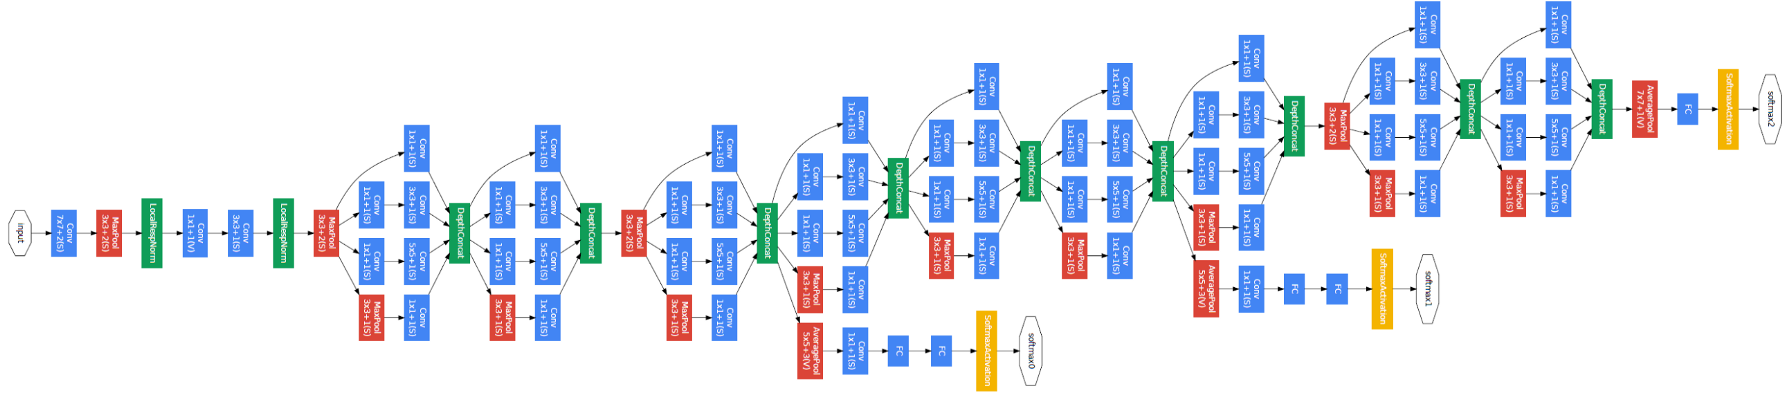
\includegraphics[width=1\linewidth]{images/googlenet}
	\caption[Arquitectura InceptionNet]{Arquitectura InceptionNet}
	\label{fig:googlenet}
\end{figure}

\begin{figure}
	\centering
	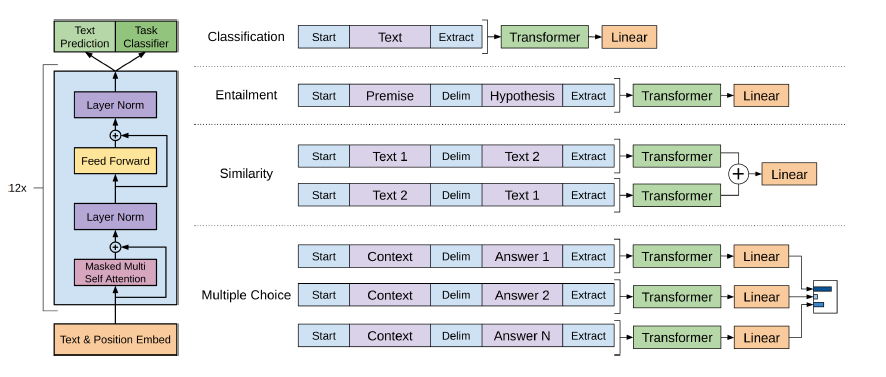
\includegraphics[width=1\linewidth]{images/gpt2}
	\caption[Arquitectura GPT2]{}
	\label{fig:gpt2}
\end{figure}

La forma más simple de utilizar estas redes para hacer transferencia de aprendizaje es haciendo inferencia directamente a partir de ellas, es decir, descargarlas, brindarles datos de entrada y realizar una pasada hacia adelante con el fin de obtener las salidas. Otra opción es reentrenar a la red con un conjunto de datos propio, de manera de extraer las características aprendidas por la misma y poder refinar sus pesos con un conjunto de entrenamiento que se entiende será más similar a las imágenes con las que luego se realizarán predicciones. Por último, otra manera de reentrenar estas redes es quitando la capa de salida y agregando capas conectadas a la anteúltima capa de la red. Esto permite tanto agregar capas extra sin entrenar a la red como cambiar las predicciones esperadas utilizando una capa de salida diferente a la inicial.
